
% VoMi uncomment this to learn the width of our page (for matlab to properly plot stuff)
%\showthe\textwidth % For single column documents
%\showthe\columnwidth % For multiple column documents

\chapter{Week 14 -- Offline SoH Estimation}

% The paper headers



% As a general rule, do not put math, special symbols or citations
% in the abstract or keywords.
\section{Abstract}
This report presents an implementation and results of two offline state of health evaluation methods. The assignment provided measured data from a single cell after 0, 12000 and 24000 cycles, namely the impedance data from Electrochemical Impedance Spectroscopy (EIS) and the voltage-capacity dependence for calculation of Differential Voltage (DV) and Incremental capacity (IC) curves. Visualized samples from individual experiments were compared both qualitatively and quantitatively.


\section{EIS}

\begin{figure}[hbp]
    \centering
\begin{subfigure}{0.49\textwidth}
    \centering
    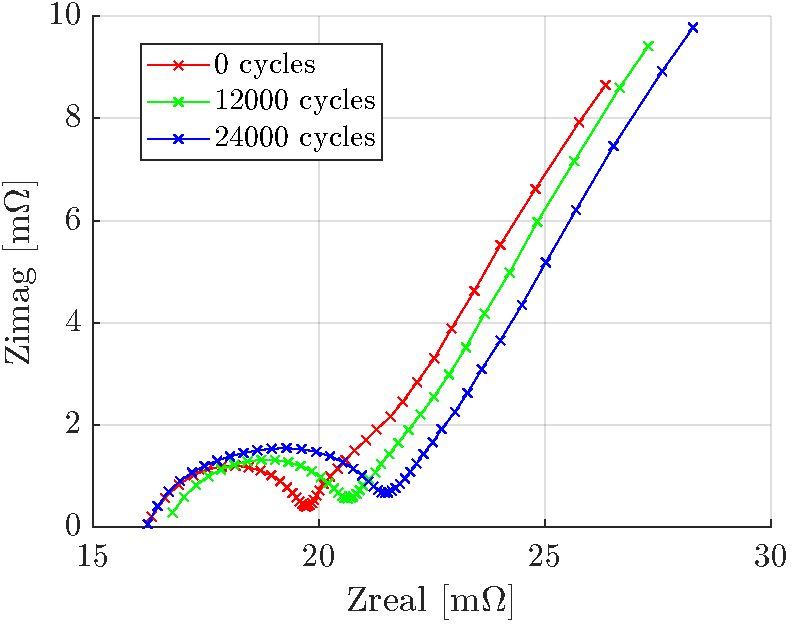
\includegraphics[width=\textwidth]{figures/14/EIS-impedance-measured.pdf}
    \caption{Measured samples.}
    \label{fig:14-EIS-measured}
    \end{subfigure}
    \hfill
    \begin{subfigure}{0.49\textwidth}
    \centering
    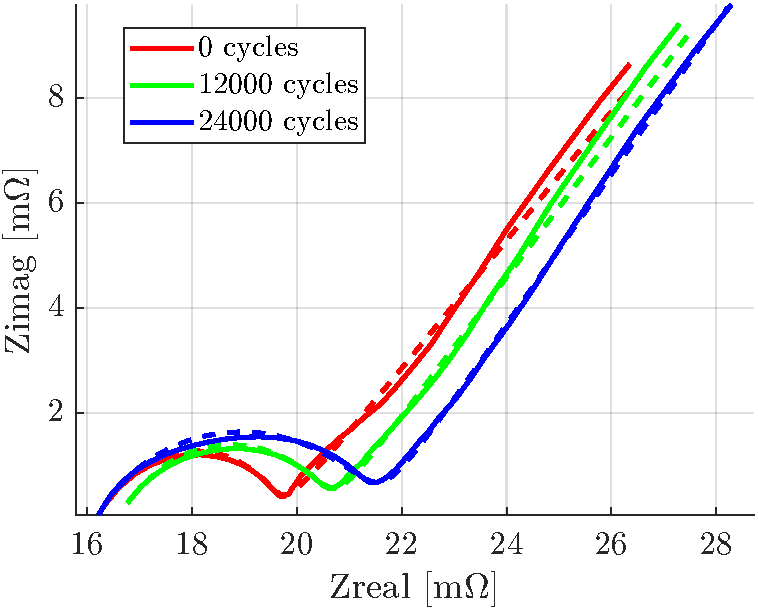
\includegraphics[width=\textwidth]{figures/14/EIS-impedance-fit.pdf}
    \caption{Measured and fitted curves.}
    \label{fig:14-EIS-fit}
    \end{subfigure}
    
    \caption{Evolution of EIS curves as the cell under test ages.}
    \label{fig:14-EIS}
\end{figure}

All provided EIS data correspond to SoC of 60 \%. The data was preprocessed according to the standard method -- first remove samples with $\Im Z > 0$ (as the indictive character is more influenced by parasitic properties of wires and cell tabs rather than the battery itself) and then flip the sign of $\Im Z$ in the remaining samples to get a plot in the first quadrant. The remaining measured samples are shown in Fig. \ref{fig:14-EIS-measured}. There is a noticeable trend that the inflexion point moves right to higher real parts of the total impedance. It should be noted that the available data does not show a noticeable change in $R_0$ over the cell's lifetime. This indicates that the resistance of conductors stayed mostly unchanged, and rather only the electrochemical part was subject to degradation.

To fit the provided EIS curves, the parameterized impedance of a equivalent circuit proposed in \cite{fernandez} was calculated. It was composed a series interconnection of blocks
\begin{enumerate}
    \item real impedance $R_0$,
    \item $R_{SEI}$ in parallel to a constant phase element (CPE),
    \item $R_{ct}$ in series with semi-infinite Warburg, the whole branch in parallel to a CPE.
\end{enumerate}

\begin{table}[]
    \centering
    \begin{tabular}{c||c|c|c|c||c|c|c}
        Number of cycles & $R_0$ [m$\Omega$] & $R_{SEI}$ [m$\Omega$] & $R_{ct}$ [m$\Omega$] & $R_{W}$ [m$\Omega$] & CL [\%] & LLI [\%] & LAM [\%] \\ \hline \hline
        0 & 16.36 & 3.28 & 3.91 & 5.57 & 0.00 & 0.00 & 0.00 \\
        12000 & 16.71 & 3.93 & 6.19 & 5.98 & 2.13 & 40.82 & 7.38 \\
        24000 & 16.21 & 5.32 & 4.80 & 8.08 & -0.94 & 40.87 & 45.15 \\

    \end{tabular}
    \caption{Equivalent circuit parameters fitted from EIS measurements.}
    \label{tab:14-eis}
\end{table}

Fitted curves are shown in Fig. \ref{fig:14-EIS-fit} and parameters are important parameters are listed in Table \ref{tab:14-eis}. The last three columns additionally include the evaluated "growth in percentage" $G_{EIC}$ metric for individual degradation modes, namely conductivity loss (CL), Lithium loss inventory (LLI) and loss of active material (LAM). Analyzing the table more closely, due to the negligible variance of $R_0$, the conductivity loss is a very unlikely degradation mode. On the other hand the growth of SEI (Solid Electrolyte Interface) resistance $R_{SEI}$ and charge transfer resistance $R_{ct}$ hint at significant loss of Lithium inventory (LLI). Finally, the increasing Warburg resistance $R_W$ hints at gradual loss of active material (LAM) degradation mode.




\section{IC/DV Analysis}

A similar analysis can be performed using the time-domain data from a charging half-cycle -- ideally with low charging current to obtain pseudo OCV curves, but the assignment only provided CC-CV charging with 1.5 A of current. The measured relation between cell terminal voltage and the current capacity is shown in Fig. \ref{fig:14-QU} for three distinct charging half-cycles throughout the cell's lifetime. The first obvious observation is that as the cell ages, the total capacity decreases, hence the CC-CV charging ends earlier at lower capacity.

\begin{figure}
    \centering
    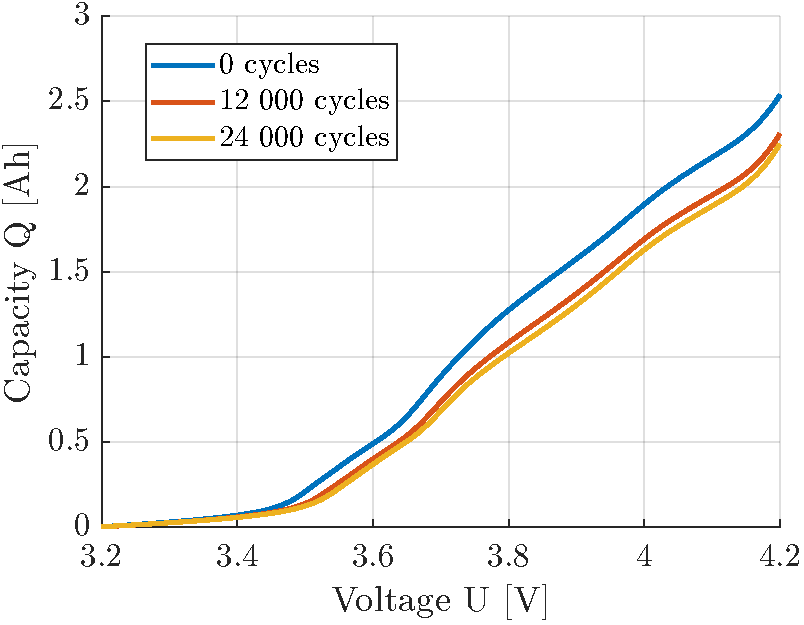
\includegraphics[width=0.5\textwidth]{figures/14/QU.pdf}
    \caption{Collected voltage-capacity data from three charging half-cycles.}
    \label{fig:14-QU}
\end{figure}

\begin{figure}[b]
\centering
\begin{minipage}{0.49\textwidth}
    \centering
    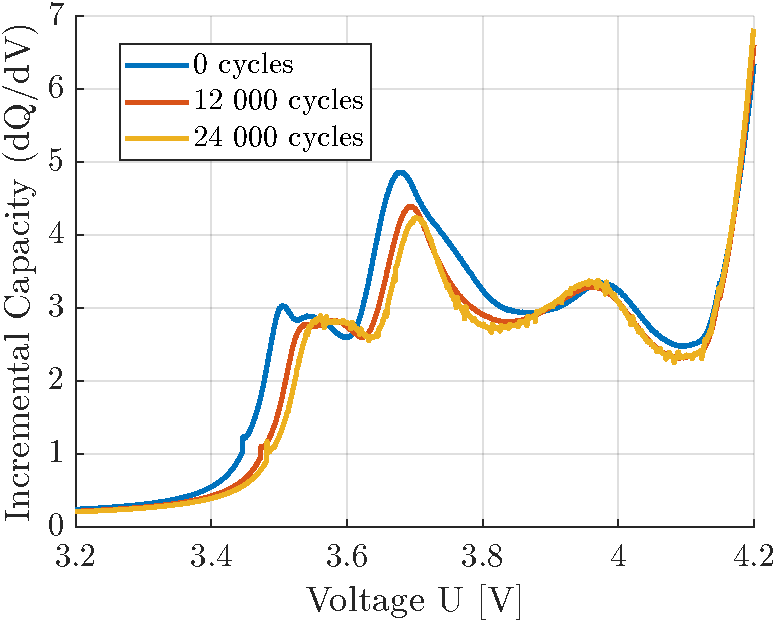
\includegraphics[width=\textwidth]{figures/14/IC.pdf}
    \caption{Evolution of Incremental capacity (IC) during cell's lifetime.}
    \label{fig:14-IC}
\end{minipage}
\hfill
\begin{minipage}{0.49\textwidth}
    \centering
    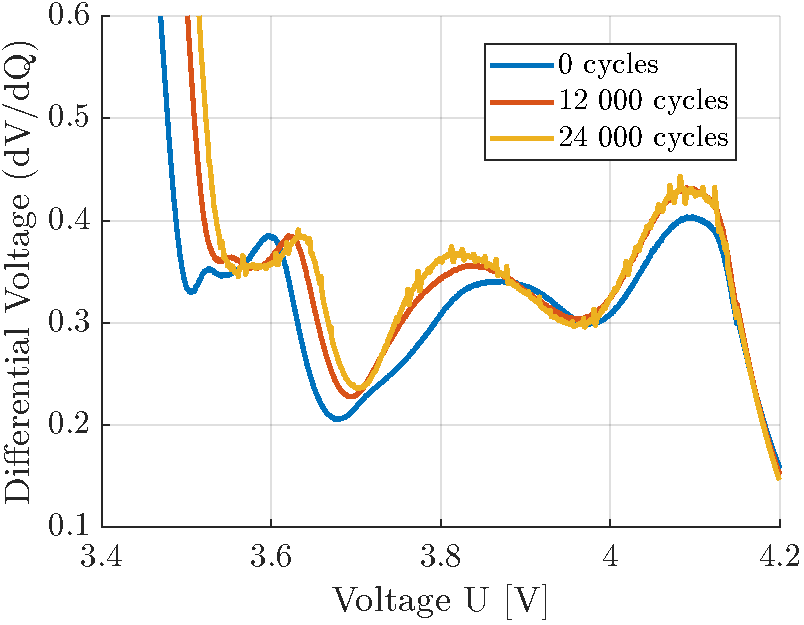
\includegraphics[width=\textwidth]{figures/14/DV.pdf}
    \caption{Evolution of Differential voltage (DV) during cell's lifetime.}
    \label{fig:14-DV}
\end{minipage}
\end{figure}

To facilitate the calculation of Incremental capacity and Differential Voltage curves, the data was preprocessed to suppress measurement noise using a Savitzky-Golay Filter of order 3 and frame length 501 samples. Subsequently duplicated neighbouring measurements resulting in division by zero were eliminated.
Both curves for all experiments are shown in Fig. \ref{fig:14-IC} and \ref{fig:14-DV}, respectively. Again, there are some clear differences between the reference curves corresponding to 0 cycles and curves corresponding to points later in the cell's life -- for example the DV curve in Fig. \ref{fig:14-DV} gets overall higher whilst the IC curve in \ref{fig:14-IC} overall moves down since as the total capacity decreases with cell's age, lower amount of charge is needed to increase the terminal voltage.

Using formulae from \cite{fernandez}, degradation mode indicators for CL, LLI and LAM listed in Table \ref{tab:14-icdv} were calculated. Obtained results roughly match the conclusion from EIS (see \ref{tab:14-eis}) -- the cell aged in a way that did not influence the resistance of conductors, whereas both LLI and LAM are noticeable.







\begin{table}[]
    \centering
    \begin{tabular}{c||c|c|c}
        Number of cycles & CL [\%] & LLI [\%] & LAM [\%] \\ \hline \hline
        0 & 0.00e+00 & 0.00 & 0.00 \\
        12000 & 2.72e-05 & 8.98 & 9.64 \\
        24000 & 1.53e-02 & 11.42 & 12.89 \\

    \end{tabular}
    \caption{Degradation modes identified using IC/DV curves.}
    \label{tab:14-icdv}
\end{table}


